\section{Experiment}\label{sec:experiment}

\begin{table}[t]
  \centering
  \caption{Best-of-$N$ selection accuracy. \textbf{BBF}: black-box friendly. For non-RCS methods, \textbf{bold} = statistically significant improvement over best RCS ($p{<}0.05$, paired t-test). For RCS methods (shaded), \textbf{bold} = best RCS variant per column. Greedy averages use unrounded values. Additional results in Appendix Table~\ref{tab:ranking-addition}.}
  \label{tab:ranking}
  \resizebox{\columnwidth}{!}{
  \begin{tabular}{ll |c| ccccc | c}
    \toprule
    \textbf{Model} & \textbf{Method} & \textbf{BBF}
    & \textbf{SciQ} & \textbf{GPQA} 
    & \textbf{Arithmetics} & \textbf{GSM8K} & \textbf{Form.Log.} 
    & \textbf{Average}
    \\
    \midrule
    \multirow{13}{*}{Qwen2.5-3B}
    & Greedy & \ding{51} & 59.3 & 20.9 & 89.0 & 65.0 & 34.9 & 54.3\\
    & Oracle & \ding{51} & 80.8$\pm$0.7	& 51.0$\pm$2.9 & 99.5$\pm$0.5	& 93.1$\pm$0.8 &	73.5$\pm$5.7 & 79.6\\
    \cmidrule(lr){2-9}
    & NLL & \ding{55}& 59.4$\pm$0.7 & 15.7$\pm$2.4 & 36.0$\pm$0.9 & 25.0$\pm$3.1 & 23.0$\pm$2.7 & 31.8 \\
    & ANLL & \ding{55}& 59.2$\pm$0.5 & 15.9$\pm$2.2 & 36.0$\pm$1.3 & 24.9$\pm$3.3 & 22.8$\pm$3.0 & 31.8 \\
    & SC & \ding{51}   & 64.4$\pm$0.6 & 21.4$\pm$0.6 & 78.7$\pm$3.3 & 52.8$\pm$1.3 & 40.5$\pm$2.1 & 51.6 \\
    & CE & \ding{55}   & 64.0$\pm$0.5 & 16.8$\pm$1.7 & 80.3$\pm$4.3 & 53.3$\pm$2.8 & 41.3$\pm$0.8 & 51.1 \\
    & ModeX & \ding{51} & 62.3$\pm$0.1	&18.1$\pm$2.3	&48.5$\pm$2.3&	33.3$\pm$3.1	&25.1$\pm$2.6 & 37.5\\
    & SCW & \ding{51} & 64.5$\pm$0.8 & 23.0$\pm$0.3 & 83.7$\pm$3.3 & 64.3$\pm$2.3 & 44.4$\pm$0.8 & 56.0 \\
    &\cellcolor{green!15} RCS$_\text{medoid}$ &\cellcolor{green!15} \ding{51} &\cellcolor{green!15} 65.2$\pm$1.0 &\cellcolor{green!15} 23.8$\pm$0.5 &\cellcolor{green!15} 81.7$\pm$3.0 &\cellcolor{green!15} 63.6$\pm$2.6 &\cellcolor{green!15} 43.6$\pm$1.6 &\cellcolor{green!15} 55.6 \\
    &\cellcolor{green!15} RCS$_\text{uni}$ &\cellcolor{green!15} \ding{51} & \cellcolor{green!15} \textbf{65.6$\pm$0.4} & \cellcolor{green!15} 23.1$\pm$2.2 & \cellcolor{green!15} \textbf{85.7$\pm$3.2} &\cellcolor{green!15} \textbf{65.8$\pm$3.1} &\cellcolor{green!15} \textbf{44.7$\pm$1.2} &\cellcolor{green!15} \textbf{57.0} \\
    & \cellcolor{green!15} RCS$_\text{freq}$ &\cellcolor{green!15} \ding{51} &\cellcolor{green!15} 64.8$\pm$0.7 &\cellcolor{green!15} 22.8$\pm$0.5 &\cellcolor{green!15} 82.8$\pm$4.6 &\cellcolor{green!15} 59.7$\pm$1.6 &\cellcolor{green!15} 43.4$\pm$1.7 &\cellcolor{green!15} 54.7 \\
    & \cellcolor{green!15} RCS$_\text{cosine}$ &\cellcolor{green!15} \ding{51} &\cellcolor{green!15} \textbf{65.6$\pm$0.6} &\cellcolor{green!15} \textbf{24.2$\pm$1.8} &\cellcolor{green!15} 85.2$\pm$4.5 &\cellcolor{green!15} 65.0$\pm$2.8 &\cellcolor{green!15} \textbf{44.7$\pm$1.2} &\cellcolor{green!15} 56.9 \\
    & \cellcolor{green!15} RCS$_\text{prob}$ &\cellcolor{green!15} \ding{55} &\cellcolor{green!15} 65.5$\pm$0.6 &\cellcolor{green!15} 22.5$\pm$2.4 &\cellcolor{green!15} 84.2$\pm$4.0&\cellcolor{green!15} 63.4$\pm$1.8 &\cellcolor{green!15} 43.9$\pm$1.2 &\cellcolor{green!15} 55.9 \\
    \midrule

    % \multirow{11}{*}{Qwen2.5-7B}
    % & Greedy & \ding{51}& 64.1 & 20.5 & 97.0 & 88.3 & 43.6 & 63.1\\
    % & Oracle & \ding{51} & 	82.0$\pm$1.1 &	49.9$\pm$1.6 & 	100.0$\pm$0.0	& 94.6$\pm$0.8	& 67.7$\pm$2.5 & 78.8 \\
    % \cmidrule(lr){2-9}
    % & NLL & \ding{55}& 66.4$\pm$0.1 & 18.3$\pm$1.3 & 47.3$\pm$5.7 & 32.7$\pm$4.3 & 25.7$\pm$0.5 & 38.1 \\
    % & ANLL & \ding{55}& 66.2$\pm$0.4 & 18.1$\pm$0.9 & 47.0$\pm$5.6 & 32.7$\pm$4.4 & 25.9$\pm$0.5 & 38.0 \\
    % & SC & \ding{51}   & \textbf{70.3$\pm$0.9} & 22.1$\pm$4.2 & 74.3$\pm$2.0 & 52.3$\pm$2.0 & \textbf{48.4$\pm$0.0} & 53.5 \\
    % & CE & \ding{55}   & \textbf{70.4$\pm$0.4} & 21.6$\pm$3.8 & \textbf{75.5$\pm$4.0} & 51.9$\pm$3.1 & \textbf{48.7$\pm$1.2} & 53.6 \\
    % & ModeX & \ding{51} & 69.0$\pm$0.6	&21.6$\pm$1.6	&54.3$\pm$5.1	&37.6$\pm$3.3&	35.2$\pm$2.6& 43.5\\
    % &\cellcolor{green!15} RCS$_\text{medoid}$ &\cellcolor{green!15} \ding{51} &\cellcolor{green!15} 70.1$\pm$0.6 &\cellcolor{green!15} 25.0$\pm$1.3 &\cellcolor{green!15} 77.5$\pm$3.6 &\cellcolor{green!15} 57.5$\pm$2.6 &\cellcolor{green!15} \textbf{49.2$\pm$2.9} &\cellcolor{green!15} 55.9 \\
    % &\cellcolor{green!15} RCS$_\text{uni}$ &\cellcolor{green!15} \ding{51} & \cellcolor{green!15} 70.2$\pm$0.2 & \cellcolor{green!15}\textbf{27.1$\pm$1.7} &\cellcolor{green!15} 77.5$\pm$2.3 &\cellcolor{green!15} 61.6$\pm$2.8 &\cellcolor{green!15} \textbf{49.2$\pm$3.2} &\cellcolor{green!15} 57.1 \\
    % & \cellcolor{green!15} RCS$_\text{freq}$ &\cellcolor{green!15} \ding{51} &\cellcolor{green!15} \textbf{70.3$\pm$0.5} &\cellcolor{green!15} 25.9$\pm$1.8 &\cellcolor{green!15} 76.7$\pm$1.4 &\cellcolor{green!15} 56.0$\pm$2.1 &\cellcolor{green!15} 47.9$\pm$2.4 &\cellcolor{green!15} 55.4 \\
    % & \cellcolor{green!15} RCS$_\text{prob}$ &\cellcolor{green!15} \ding{55} &\cellcolor{green!15} 70.0$\pm$0.4 &\cellcolor{green!15} \textbf{27.1$\pm$2.4} &\cellcolor{green!15} \textbf{77.7$\pm$1.9} &\cellcolor{green!15} \textbf{62.1$\pm$3.1} &\cellcolor{green!15} \textbf{49.2$\pm$3.2} & \cellcolor{green!15}\textbf{57.2} \\
    % \midrule

    % \multirow{13}{*}{Llama3.2-3B}
    % & Greedy & \ding{51}& 55.6 & 23.0 & 96.0 & 79.7 & 34.9 & 58.3 \\
    % & Oracle & \ding{51} & 79.8$\pm$0.4 &	52.5$\pm$1.5 & 99.8$\pm$0.3	& 92.6$\pm$0.3	& 71.4$\pm$4.4 & 79.2\\
    % \cmidrule(lr){2-9}
    % & NLL & \ding{55}& 53.6$\pm$1.1 & 20.2$\pm$3.2 & 86.5$\pm$1.3 & 74.3$\pm$1.5 & \textbf{33.3$\pm$2.1} & 53.6 \\
    % & ANLL & \ding{55}& 53.6$\pm$0.5 & 19.7$\pm$0.5 & 88.5$\pm$2.6 & 73.9$\pm$2.4 & \textbf{29.9$\pm$6.0} & 53.1 \\
    % & SC & \ding{51}   & \textbf{58.8$\pm$1.1} & 17.4$\pm$2.6 & \textbf{97.5$\pm$1.3} & 78.0$\pm$0.8 & 16.1$\pm$3.2 & 53.6 \\
    % & CE & \ding{55}   & \textbf{59.3$\pm$0.6} & 20.9$\pm$2.2 & \textbf{97.3$\pm$1.3} & 78.5$\pm$0.8 & 17.5$\pm$2.7 & 54.7 \\
    % & ModeX & \ding{51} & 53.2$\pm$0.6&	18.1$\pm$2.1	&70.0$\pm$2.3	&62.6$\pm$2.1	&16.9$\pm$0.5& 44.2\\
    % & SCW & \ding{51} & 59.5$\pm$1.0 & 25.4$\pm$0.9 & 94.0$\pm$1.3 & 80.5$\pm$1.5 & 20.6$\pm$2.4 & 56.0 \\
    % &\cellcolor{green!15} RCS$_\text{medoid}$ &\cellcolor{green!15} \ding{51} &\cellcolor{green!15} \textbf{60.0$\pm$1.2} &\cellcolor{green!15} 25.6$\pm$0.8 &\cellcolor{green!15} \textbf{98.3$\pm$1.0} &\cellcolor{green!15} 80.5$\pm$1.5 &\cellcolor{green!15} 19.6$\pm$3.7 &\cellcolor{green!15} 56.8 \\
    % &\cellcolor{green!15} RCS$_\text{uni}$ &\cellcolor{green!15} \ding{51} &\cellcolor{green!15} 59.5$\pm$0.8 &\cellcolor{green!15} 25.0$\pm$0.8 &\cellcolor{green!15} 98.2$\pm$1.0 &\cellcolor{green!15} 80.5$\pm$1.5 &\cellcolor{green!15} 20.4$\pm$3.2 &\cellcolor{green!15} 56.7 \\
    % & \cellcolor{green!15} RCS$_\text{freq}$ &\cellcolor{green!15} \ding{51} &\cellcolor{green!15} 59.8$\pm$1.0 &\cellcolor{green!15} 25.4$\pm$0.9 &\cellcolor{green!15} 98.2$\pm$1.0 &\cellcolor{green!15} 79.4$\pm$1.3 &\cellcolor{green!15} 18.0$\pm$3.7 &\cellcolor{green!15} 56.2 \\
    % & \cellcolor{green!15} RCS$_\text{cosine}$ &\cellcolor{green!15} \ding{51} &\cellcolor{green!15} 59.8$\pm$1.2 &\cellcolor{green!15} 25.2$\pm$1.2 &\cellcolor{green!15} 98.0$\pm$0.9 &\cellcolor{green!15} 81.1$\pm$1.6 &\cellcolor{green!15} 20.6$\pm$3.6 &\cellcolor{green!15} 56.9 \\
    % & \cellcolor{green!15} RCS$_\text{prob}$ &\cellcolor{green!15} \ding{55} &\cellcolor{green!15} 59.6$\pm$0.8 &\cellcolor{green!15} \textbf{26.2$\pm$1.3} &\cellcolor{green!15} 97.5$\pm$0.8 &\cellcolor{green!15} \textbf{84.1$\pm$0.8} &\cellcolor{green!15} \textbf{33.1$\pm$3.2} &\cellcolor{green!15} \textbf{60.2} \\
    % \midrule

    \multirow{13}{*}{Llama3.1-8B}
    & Greedy & \ding{51}& 63.1 & 25.5 & 89.5 & 88.3 & 34.9 & 60.8\\
    & Oracle & \ding{51} & 85.1$\pm$0.4	& 56.3$\pm$1.3 & 99.3$\pm$0.3	& 94.6$\pm$0.8	& 74.1$\pm$1.2 & 81.9 \\
    \cmidrule(lr){2-9}
    & NLL & \ding{55}& 61.0$\pm$0.5 & 20.4$\pm$0.8 & 73.3$\pm$2.8 & 69.0$\pm$0.5 & 33.9$\pm$2.8 & 51.5 \\
    & ANLL & \ding{55}& 61.1$\pm$0.5 & 18.7$\pm$0.9 & 73.5$\pm$4.1 & 68.7$\pm$1.6 & 33.1$\pm$2.4 & 51.0 \\
    & SC & \ding{51}   & \textbf{67.3$\pm$0.7} & 16.8$\pm$1.8 & 78.3$\pm$3.0 & 66.0$\pm$2.3 & 31.7$\pm$2.1 & 52.0 \\
    & CE & \ding{55}   & 66.8$\pm$0.9 & 18.5$\pm$1.1 & 81.0$\pm$3.8 & 67.5$\pm$1.3 & 32.3$\pm$1.7 & 53.2 \\
    & ModeX & \ding{51} &	63.1$\pm$1.2&	17.8$\pm$1.1&	55.3$\pm$2.5	&48.4$\pm$3.9	&25.1$\pm$2.6 & 41.9\\
    & SCW & \ding{51} & 67.7$\pm$1.0 & 26.8$\pm$0.8 & 82.2$\pm$2.8 & 71.4$\pm$2.9 & 36.8$\pm$1.7 & 57.0 \\
    &\cellcolor{green!15} RCS$_\text{medoid}$ &\cellcolor{green!15} \ding{51} &\cellcolor{green!15} 68.0$\pm$0.9 &\cellcolor{green!15} 26.4$\pm$0.9 &\cellcolor{green!15} 86.5$\pm$1.5 &\cellcolor{green!15} 71.4$\pm$2.8 &\cellcolor{green!15} 37.8$\pm$0.9 &\cellcolor{green!15} 58.0 \\
    &\cellcolor{green!15} RCS$_\text{uni}$ &\cellcolor{green!15} \ding{51} &\cellcolor{green!15} \textbf{68.1$\pm$0.7} &\cellcolor{green!15} 26.9$\pm$1.0 &\cellcolor{green!15} \textbf{88.5$\pm$0.5} &\cellcolor{green!15} 72.8$\pm$3.0 &\cellcolor{green!15} \textbf{39.4$\pm$0.9} &\cellcolor{green!15} \textbf{59.1} \\
    & \cellcolor{green!15} RCS$_\text{freq}$ &\cellcolor{green!15} \ding{51} &\cellcolor{green!15} 67.6$\pm$1.1 &\cellcolor{green!15} 26.9$\pm$1.0 &\cellcolor{green!15} 83.7$\pm$2.3 & \cellcolor{green!15} 68.9$\pm$1.9 & \cellcolor{green!15} 34.9$\pm$0.8& \cellcolor{green!15} 56.4 \\
    & \cellcolor{green!15} RCS$_\text{cosine}$ &\cellcolor{green!15} \ding{51} &\cellcolor{green!15} \textbf{68.1$\pm$0.7} &\cellcolor{green!15} 27.3$\pm$0.8 &\cellcolor{green!15} 87.7$\pm$1.2 &\cellcolor{green!15} 72.8$\pm$2.3 &\cellcolor{green!15} \textbf{39.4$\pm$0.9} &\cellcolor{green!15} \textbf{59.1} \\
    & \cellcolor{green!15} RCS$_\text{prob}$ &\cellcolor{green!15} \ding{55} &\cellcolor{green!15} 67.9$\pm$1.1 &\cellcolor{green!15} \textbf{27.5$\pm$0.9} &\cellcolor{green!15} 85.2$\pm$0.6 &\cellcolor{green!15} \textbf{75.6$\pm$1.0} &\cellcolor{green!15} 36.8$\pm$2.6 &\cellcolor{green!15} 58.6 \\
    % \midrule

    % \multirow{11}{*}{Gemma2-9B}
    % & Greedy & \ding{51}& 67.6 & 22.6 & 96.0 & 69.0 & 52.4 & 62.0\\
    % & Oracle & \ding{51} & 84.6$\pm$0.6 &	48.5$\pm$4.2 & 98.2$\pm$0.6	& 95.3$\pm$0.3	& 77.8$\pm$5.7 & 80.9\\
    % \cmidrule(lr){2-9}
    % & NLL & \ding{55} & 72.9$\pm$1.1 & \textbf{25.6$\pm$1.1} & 94.8$\pm$1.3 & 67.9$\pm$1.1 & 48.1$\pm$2.8 & 61.9 \\
    % & ANLL & \ding{55}& 66.3$\pm$0.9 & 21.2$\pm$2.3 & 96.0$\pm$1.0 & \textbf{73.1$\pm$0.9} & 50.0$\pm$0.8 & 61.3 \\
    % & SC & \ding{51}   & \textbf{73.9$\pm$0.2} & 19.7$\pm$0.9 & \textbf{97.3$\pm$0.3} & \textbf{72.9$\pm$3.5} & \textbf{51.6$\pm$0.8} & 63.1 \\
    % & CE & \ding{55}   & \textbf{73.6$\pm$0.6} & 18.6$\pm$0.5 & \textbf{97.5$\pm$0.0} & \textbf{73.1$\pm$3.7} & \textbf{52.1$\pm$1.7} & 63.0 \\
    % & ModeX & \ding{51} & 71.7$\pm$0.2	&19.5$\pm$2.2	&92.7$\pm$2.8	&62.6$\pm$1.5&	\textbf{49.2$\pm$4.2}& 59.1\\
    % &\cellcolor{green!15} RCS$_\text{medoid}$ &\cellcolor{green!15} \ding{51} &\cellcolor{green!15} \textbf{74.2$\pm$0.4} &\cellcolor{green!15} 24.4$\pm$1.4 &\cellcolor{green!15} 97.2$\pm$0.6 &\cellcolor{green!15} 72.9$\pm$3.5 &\cellcolor{green!15} 52.6$\pm$0.9 &\cellcolor{green!15} 64.3 \\
    % & \cellcolor{green!15} RCS$_\text{uni}$ &\cellcolor{green!15} \ding{51} &\cellcolor{green!15} 74.0$\pm$0.4 & \cellcolor{green!15}25.9$\pm$0.5 &\cellcolor{green!15}97.2$\pm$0.6 &\cellcolor{green!15} 73.8$\pm$2.8 &\cellcolor{green!15} \textbf{52.9$\pm$2.0} &\cellcolor{green!15} 64.8 \\ 
    % & \cellcolor{green!15} RCS$_\text{freq}$ &\cellcolor{green!15} \ding{51} &\cellcolor{green!15} 73.9$\pm$0.5 &\cellcolor{green!15} 25.7$\pm$0.6 &\cellcolor{green!15} \textbf{97.3$\pm$0.3} &\cellcolor{green!15} 72.6$\pm$3.7 &\cellcolor{green!15} 51.8$\pm$1.2 &\cellcolor{green!15} 64.3 \\
    % & \cellcolor{green!15} RCS$_\text{prob}$ &\cellcolor{green!15} \ding{55} &\cellcolor{green!15} \textbf{74.2$\pm$0.5} &\cellcolor{green!15} \textbf{26.3$\pm$0.6} &\cellcolor{green!15} \textbf{97.3$\pm$0.3} &\cellcolor{green!15} \textbf{75.1$\pm$3.5} &\cellcolor{green!15} 52.4$\pm$0.8 &\cellcolor{green!15} \textbf{65.1} \\
    
    \bottomrule
  \end{tabular}
  }
\end{table}

% ===
\subsection{Experiment Setup}\label{sec:experiment-setup}

\paragraph{Datasets.} We use seven established benchmarks covering both short-form question-answering and long-form reasoning tasks with different answer formats: (1) Short-form QA: \textbf{SciQ}~\citep{welbl2017crowdsourcing} and GPQA Diamond (\textbf{GPQA}~\citep{rein2024gpqa}), (2) Long-form Math Reasoning: \textbf{Arithmetics}~\citep{choi2025debate}, \textbf{GSM8K} \citep{cobbe2021training}, and (3) Long-form QA multiple choice: MMLU Formal Logic (\textbf{Form.Log.}~\citep{hendrycks2020aligning}), \textbf{MMLU-Pro}~\citep{wang2024mmlu}, BigBenchHard (\textbf{BBH-Date}, \textbf{BBH-Navigate}~\citep{suzgun2023challenging}).

\paragraph{Models.} We evaluate on five popular open-weight models from distinct families: Qwen2.5-3B, 7B~\citep{yang2025qwen25}, Llama3.2-3B, Llama3.1-8B~\citep{grattafiori2024llama}, and Gemma2-9B~\citep{team2024gemma}. 
% We refer to them as Falcon3, Gemma2, Llama3.1, and Llama3.2.
% Qwen2.5-1.5B, 3B, 7B
% Falcon3-7B~\citep{almazrouei2023falcon}

\paragraph{Baselines.} 

We compare our method against the following baselines, which require only single generation pass:
(1) \textbf{NLL}~\citep{nguyen2025probabilities}, which selects answers with the highest likelihood based on negative log-likelihood;
(2) \textbf{ANLL}~\citep{guerreiro2022looking}, which uses average negative log-likelihood for length-normalized scoring;
(3) \textbf{Self-Consistency (SC)}~\citep{wang2022self}, selecting the most frequent answer; (4) \textbf{Self-Certainty (CE)}~\citep{kang2025scalable}, which ranks answers by combining frequency and model confidence using Borda Voting; (5) \textbf{ModeX}~\citep{choi2026modex}, which applies spectral clustering over full reasoning trajectories and selects answers from the resulting cluster centroids; and (6) \textbf{SCW}~\citep{jain2023sc}, which embeds full reasoning trajectories, computes pairwise cosine similarities, groups scores by unique reasoning path, and selects the highest-scoring group.
% ---------------
\begin{figure}[ht]
    \centering
    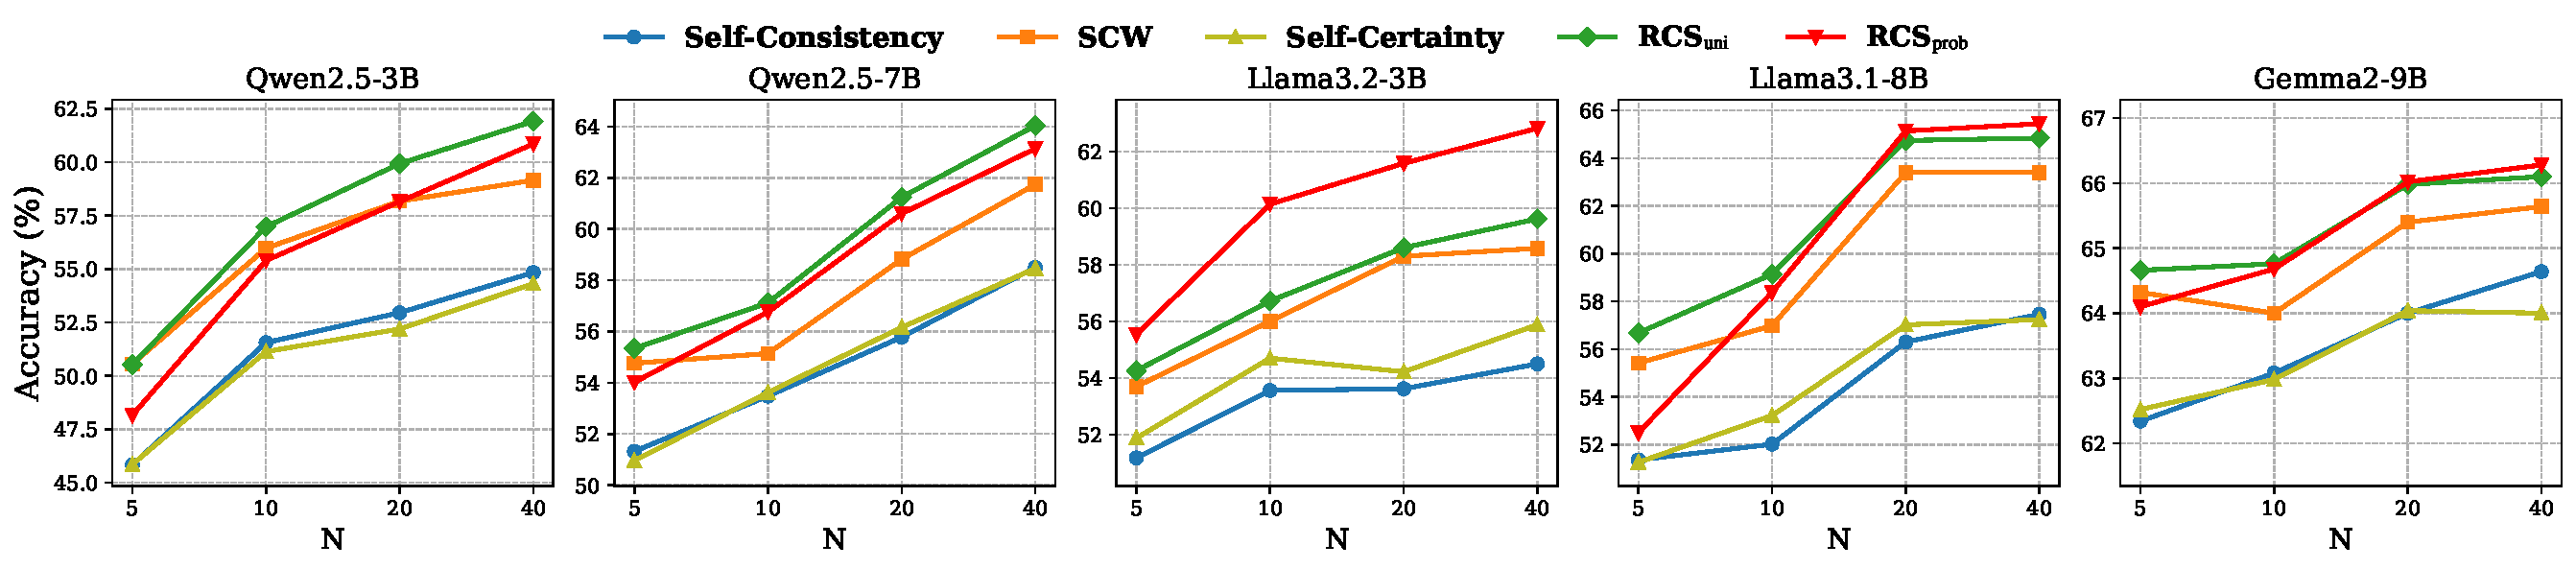
\includegraphics[width=\textwidth]{plots/scaling_methods_v6.pdf}
    \caption{
    Average performance over five benchmarks for different numbers of sampling responses $N$. Each subplot corresponds to an LLM backbone, showing how accuracy changes with increasing $N$.}
    \label{fig:scaling}
\end{figure}
% -----------
We report four RCS variants (Table~\ref{tab:rds_variants}): RCS$_\text{uni}$, RCS$_\text{freq}$, RCS$_\text{cosine}$ (per-sample cosine-similarity weights applied to final-answer embeddings), and RCS$_\text{prob}$ (using ANLL as a length-normalized probability proxy). We also report RCS$_\text{medoid}$ (uniform, unweighted) as a discrete baseline. All RCS variants use \texttt{all-MiniLM-L6-v2}~\citep{reimers2019sentence}. We sample $N{=}10$ responses (also $N{=}5,20,40$) at $T{=}1$ via vLLM~\citep{kwon2023efficient}; results are mean$\pm$std over three seeds. Additional details are in Appendix~\ref{app:details}.

% and investigate clean-answer setting in Section~\ref{sec:ablation}. 
% \paragraph{Evaluation Protocol.} For all methods, we measure accuracy (\%) between the selected answer and the ground-truth. A generation is deemed correct via exact match on long-form reasoning tasks or ROUGE-L F1 $>$ 0.3 on short-form QA tasks (SciQ, GPQA), exactly as in prior work~\citep{kuhn2023semantic, nguyen2025probabilities}. We include all model outputs, including empty or degenerate responses, to reflect real-world noisy generation settings.

% \paragraph{Sampling and Implementation.}
% We sample $N$ responses per question using multinomial sampling with temperature $T{=}1$ via vLLM~\citep{kwon2023efficient}. Unless otherwise stated, we use $N{=}10$, and additionally explore larger budgets with $N{=}5, 20, 40$. We use 5-shot prompting~\citep{brown2020language} for short-form QA and Chain-of-Thought prompting~\citep{wei2022chain} for long-form tasks. For CE, we follow the original setup and set $p{=}0.3$. 
% All RCS variants use the \texttt{all-MiniLM-L6-v2} sentence transformer~\citep{reimers2019sentence}. We report mean$\pm$std over three random seeds. Additional details are provided in Appendix~\ref{app:details}.

% ====
\subsection{Main Results}

\paragraph{RCS Consistently Outperforms Baselines.}

We report selection accuracy in Table~\ref{tab:ranking}. RCS variants consistently achieve the best performance across all settings. RCS$_\text{uni}$ and RCS$_\text{prob}$ rank first overall, outperforming the best baseline (CE) by 2--6\%. RCS$_\text{cosine}$ consistently ranks second among RCS variants (avg.\ 56.9--59.1), outperforming SCW (avg.\ 56.0--57.0) despite using the same pairwise cosine signals---demonstrating that the RCS Fréchet-mean framework extracts more value from the same information by bypassing the discrete grouping step. RCS$_\text{freq}$ outperforms SC by avoiding hard tie-breaking through soft semantic weighting.
Among baselines, CE is the strongest competitor. ModeX and SCW both underperform due to full-trajectory embedding collapse and, in SCW's case, the additional discrete-voting step that misses minority correct answers (Section~\ref{sec:embedding-collapse}).
Overall, results confirm that a unified geometric framework with flexible weighting distributions is both more expressive and more robust than fixed surface-form or trajectory-level aggregation.

% ==================SCALABILITY============================
\paragraph{RCS Scales Effectively with Increasing Sampling Budget.}\label{sec:scaling}

Figure~\ref{fig:scaling} shows performance as the number of sampled responses $N$ increases with only top methods are shown. We highlight $\text{RCS}_{\text{uni}}$ and $\text{RCS}_{\text{prob}}$, the best-performing variants from Table~\ref{tab:ranking} (full results in Appendix~\ref{app:sample-details}).
RCS consistently outperforms all baselines at larger $N$ (e.g., $N{=}20,40$), with gains up to +7\%. As $N$ increases, correct answers may remain in the minority; RCS recovers them by anchoring to the semantic center rather than to frequency, maintaining robustness even when correct outputs are sparse.




% =========================ABLATION=====================
\subsection{Ablation Study}\label{sec:ablation}

% In this section, we investigate the effects of hyperparameters, including the number of sampling responses $N$ and choice of embedding model $\mathbf{E}$. 
To reduce computational overhead, experiments are conducted using two representative models: Qwen2.5-3B and Llama3.2-3B.





\paragraph{RCS Enhances Multi-Agent Debate.}

\begin{table}[ht]
  \centering
  \caption{Performance on Arithmetics and Form.Log. with Multi-agent Debate. Best values are bolded. \textbf{R=0,1,2} indicate debate rounds, while \textbf{Avg.} denotes the average over all rounds. RCS$_\text{base}$ $\equiv$ RCS$_\text{uni}$ (uniform weighting).}
  \label{tab:mad_qwen2.5-3b}
  % \renewcommand{\arraystretch}{0.85}
  \resizebox{\columnwidth}{!}{
  \begin{tabular}{cll|cccc|cccc}
    \toprule
    \multirow{2}{*}{\textbf{Model}} 
    & \multirow{2}{*}{\textbf{Method}} 
    & \multirow{2}{*}{\textbf{N}} 
    & \multicolumn{4}{c|}{\textbf{Arithmetics}}
    & \multicolumn{4}{c}{\textbf{Form.Log.}} 
    % & \multicolumn{3}{c}{\textbf{MMLU-Pro}} 
    \\
    
    \cmidrule(lr){4-7} \cmidrule(lr){8-11} % \cmidrule(lr){9-11}
    
    & &
    & \textbf{R=0} & \textbf{R=1} & \textbf{R=2} & \textbf{Avg.}
    & \textbf{R=0} & \textbf{R=1} & \textbf{R=2} & \textbf{Avg.}
    % & \textbf{R=0} & \textbf{R=1} & \textbf{R=2} 
    \\
    
    \midrule
    % \multicolumn{8}{c}{\textbf{Qwen2.5-3B}} \\
    % \midrule

    \multirow{6}{*}{\rotatebox[origin=c]{90}{Qwen2.5-3B}}
    &
    SC & 10  
    & 94.5$\pm$4.0&	60.4$\pm$1.6	&34.6$\pm$5.8   & 63.1
    & 44.8$\pm$2.5&	35.3$\pm$2.9	&27.6$\pm$5.4   & 35.9
    % & 23.8$\pm$5.9&	22.9$\pm$5.8	&24.8$\pm$2.9 
    \\

    &
    \cellcolor{green!15}RCS$_\text{base}$ & \cellcolor{green!15}10
    & \cellcolor{green!15}94.3$\pm$3.7	&\cellcolor{green!15}59.5$\pm$4.1&\cellcolor{green!15}	34.0$\pm$11.0 & \cellcolor{green!15}62.6
    & \cellcolor{green!15}\textbf{46.0$\pm$2.3}	&\cellcolor{green!15}35.8$\pm$5.3	&\cellcolor{green!15}\textbf{28.8$\pm$6.0} & \cellcolor{green!15}\textbf{36.9}
    % & 25.4$\pm$7.4&	22.9$\pm$6.6&	24.4$\pm$5.8 
    \\
    &
    \cellcolor{green!15}RCS$_\text{freq}$ & 10\cellcolor{green!15}
    & \cellcolor{green!15}\textbf{95.2$\pm$3.6}&\cellcolor{green!15}	\textbf{61.4$\pm$1.2}	&\cellcolor{green!15}\textbf{34.7$\pm$5.4} & \cellcolor{green!15}\textbf{63.8 }
    & \cellcolor{green!15}44.8$\pm$2.8&\cellcolor{green!15}	\textbf{36.1$\pm$3.3}&\cellcolor{green!15}	28.7$\pm$5.5 & \cellcolor{green!15}36.5
    % & 24.8$\pm$5.9&	25.4$\pm$6.3&	26.0$\pm$3.9 
    \\

    \cmidrule(lr){2-11}
    &
    SC & 20  
    & 96.5$\pm$0.5&	24.8$\pm$3.0	&34.0$\pm$3.3 & 51.8
    & 42.3$\pm$0.5	&40.5$\pm$1.6	&35.7$\pm$1.6 & 39.5
    % & 23.8$\pm$1.3&	26.2$\pm$3.4	&25.7$\pm$2.7 
    \\
    & 
    \cellcolor{green!15}RCS$_\text{base}$ & 20\cellcolor{green!15}
    & \cellcolor{green!15}\textbf{97.7$\pm$1.0}	&\cellcolor{green!15}\textbf{27.3$\pm$3.2}	&\cellcolor{green!15}\textbf{34.5$\pm$5.1} & \cellcolor{green!15}\textbf{53.2} 
    & \cellcolor{green!15}\textbf{46.6$\pm$0.9}	&\cellcolor{green!15}\textbf{45.2$\pm$1.4}&	\cellcolor{green!15}\textbf{37.8$\pm$0.9} & \cellcolor{green!15}\textbf{43.2}
    % & 24.3$\pm$0.7&	27.6$\pm$6.7&	24.3$\pm$4.7 
    \\
    &
    \cellcolor{green!15}RCS$_\text{freq}$ & 20\cellcolor{green!15}
    & \cellcolor{green!15}97.2$\pm$0.3	&\cellcolor{green!15}26.0$\pm$2.2&\cellcolor{green!15}	34.3$\pm$4.0 & \cellcolor{green!15}52.5
    & \cellcolor{green!15}42.6$\pm$0.5&	\cellcolor{green!15}42.1$\pm$0.8&\cellcolor{green!15}	35.7$\pm$1.6 & \cellcolor{green!15}40.1
    % & 24.8$\pm$2.7&	25.2$\pm$6.1&	24.3$\pm$8.8 
    \\

    \midrule
    % \multicolumn{8}{c}{\textbf{Llama3.2-3B}} \\
    % \midrule
    \multirow{6}{*}{\rotatebox[origin=c]{90}{Llama3.2-3B}}
    &
    SC & 10  
    & 80.7$\pm$2.0	&85.6$\pm$10.7&	75.8$\pm$5.9 & 80.7
    & 31.3$\pm$2.9&	28.4$\pm$7.8	&29.5$\pm$7.7 & 29.7
    % & 16.2$\pm$2.5	&14.0$\pm$1.1	&14.0$\pm$2.9 
    \\
    &
    \cellcolor{green!15}RCS$_\text{base}$ & 10\cellcolor{green!15}
    & \cellcolor{green!15}79.1$\pm$4.3	&\cellcolor{green!15} \textbf{85.8$\pm$9.1}&\cellcolor{green!15}	\textbf{76.2$\pm$4.6} & \cellcolor{green!15}80.4
    & 	\cellcolor{green!15}\textbf{33.2$\pm$0.5}&\cellcolor{green!15}	\textbf{28.7$\pm$8.0}	&\cellcolor{green!15}\textbf{29.9$\pm$6.4} & \cellcolor{green!15}\textbf{30.6}
    % & 17.5$\pm$4.7	&14.9$\pm$2.0	&14.3$\pm$1.0 
    \\
    &
    \cellcolor{green!15}RCS$_\text{freq}$ & 10\cellcolor{green!15}
    & \cellcolor{green!15}\textbf{81.1$\pm$12.7}&	\cellcolor{green!15}85.6$\pm$10.0	&\cellcolor{green!15}\textbf{76.2$\pm$5.1} & \cellcolor{green!15}\textbf{81.0}
    & \cellcolor{green!15}32.1$\pm$2.9&	\cellcolor{green!15}28.6$\pm$8.3	&\cellcolor{green!15}29.5$\pm$16.6 & \cellcolor{green!15}30.1
    % & 15.6$\pm$4.7&	14.9$\pm$2.0	&12.7$\pm$1.1 
    \\

    \cmidrule(lr){2-11}
    &
    SC & 20  
    & 99.0$\pm$0.5&	72.2$\pm$4.1&	41.5$\pm$2.2 & 70.9
    & 13.2$\pm$0.5&	3.2$\pm$0.8	&3.7$\pm$1.7 & 6.7
    % & 21.4$\pm$3.4&	15.7$\pm$0.7	&13.8$\pm$2.0 
    \\
    &
    \cellcolor{green!15}RCS$_\text{base}$ & 20\cellcolor{green!15}
    & \cellcolor{green!15}99.0$\pm$1.0	&\cellcolor{green!15}\textbf{76.5$\pm$4.3}	&\cellcolor{green!15}\textbf{43.3$\pm$1.5} & \cellcolor{green!15}\textbf{72.9}
    & \cellcolor{green!15}\textbf{21.4$\pm$2.4}&\cellcolor{green!15}	\textbf{9.0$\pm$1.2}&\cellcolor{green!15}	\textbf{7.1$\pm$2.4}&\cellcolor{green!15}\textbf{12.5}
    % & 18.1$\pm$8.1	&18.1$\pm$4.0&	14.3$\pm$6.7 
    \\
    &
    \cellcolor{green!15}RCS$_\text{freq}$ & 20\cellcolor{green!15}
    & \cellcolor{green!15}\textbf{99.2$\pm$0.8}	&\cellcolor{green!15}73.8$\pm$3.8&\cellcolor{green!15}	42.5$\pm$2.6 & \cellcolor{green!15}71.8
    & \cellcolor{green!15}15.6$\pm$1.7	&\cellcolor{green!15}4.2$\pm$0.5&\cellcolor{green!15}	3.7$\pm$0.9 & \cellcolor{green!15}7.8
    % & 19.0$\pm$2.7&	15.7$\pm$3.4&	13.8$\pm$0.7 
    \\

    \bottomrule
  \end{tabular}}
\end{table}
% ------------
% ------
% =================
\begin{table*}[t]
\centering
\caption{Performance under (a) black-box setting ($N{=}$10) and (b) complexity comparison.}
\label{tab:clean-blackbox-complexity}
\resizebox{\linewidth}{!}{
\begin{tabular}{c c}
% ================= LEFT TABLE (a) =================
% \begin{minipage}[t]{0.70\linewidth}
% \centering
% \caption*{\vspace{1pt}(a)}
% \resizebox{\linewidth}{!}{
% \begin{tabular}{l|cc|cc}
% \toprule
% \multirow{2}{*}{\textbf{Method}} 
% & \multicolumn{2}{c|}{\textbf{Qwen2.5-3B}} 
% & \multicolumn{2}{c}{\textbf{Llama3.2-3B}} \\
% \cmidrule(lr){2-3} \cmidrule(lr){4-5}
% & \textbf{Arithmetics} & \textbf{Form.Log.} 
% & \textbf{Arithmetics} & \textbf{Form.Log.} \\
% \midrule
% NLL  & 54.2$\pm$4.3 & 29.6$\pm$5.6 & 87.0$\pm$1.0 & 38.6$\pm$4.4 \\
% ANLL & 54.0$\pm$4.0 & 29.9$\pm$6.2 & 89.5$\pm$2.3 & 38.9$\pm$5.6 \\
% SC   & 96.7$\pm$1.2 & 46.6$\pm$1.7 & 98.0$\pm$1.3 & 36.2$\pm$3.2 \\
% CE   & 96.5$\pm$0.9 & 48.4$\pm$1.1 & 97.8$\pm$1.3 & 37.8$\pm$2.9 \\
% \rowcolor{green!15}RCS$_{\text{medoid}}$ & \textbf{97.2$\pm$0.6} & 48.9$\pm$1.2 & \textbf{98.3$\pm$0.8} & 36.5$\pm$2.9 \\
% \rowcolor{green!15}RCS$_{\text{uni}}$  & 95.5$\pm$1.3 & 49.2$\pm$0.8 & 98.2$\pm$1.0 & 37.0$\pm$3.3 \\
% \rowcolor{green!15}RCS$_{\text{freq}}$ & 96.8$\pm$0.6 & \textbf{49.7$\pm$0.9} & \textbf{98.3$\pm$0.8} & 37.0$\pm$2.0 \\
% \rowcolor{green!15}RCS$_{\text{prob}}$ & 94.3$\pm$1.9 & 48.4$\pm$0.8 & 97.7$\pm$1.0 & \textbf{40.2$\pm$4.8} \\
% \bottomrule
% \end{tabular}}

% \end{minipage}

\begin{minipage}[t]{0.75\linewidth}
\centering
    \caption*{(a)}

\label{tab:blackbox}
\resizebox{\linewidth}{!}{
\begin{tabular}{l|cccc|c}
\toprule
\textbf{Method} & \textbf{GPQA} & \textbf{MMLU-Pro} & \textbf{BBH-Date} & \textbf{BBH-Navigate} & {\textbf{Avg.}}\\
\midrule
SC  & 13.1 & 47.6 & 76.8 & 39.2 & 44.2\\
\rowcolor{green!15}RCS$_\text{medoid}$ & \textbf{14.6} & \textbf{48.6} & 76.4 & 39.2 & 44.7\\
\rowcolor{green!15}RCS$_\text{base}$   & 14.1 & \textbf{48.6} & \textbf{78.0} & 40.2 & \textbf{45.2}\\
\rowcolor{green!15}RCS$_\text{freq}$   & 13.6 & 47.6 & 77.6 & \textbf{41.2} & 45.0\\
\bottomrule
\end{tabular}}
\end{minipage}


&

% ================= RIGHT SIDE (b + c stacked) =================
\begin{minipage}[t]{0.22\linewidth}
\centering

% -------- (b) Blackbox table --------
% \caption*{(b)}

% \label{tab:blackbox}
% \resizebox{\linewidth}{!}{
% \begin{tabular}{l|cc}
% \toprule
% \textbf{Method} & \textbf{AIME25} & \textbf{MMLU-Pro} \\
% \midrule
% SC  & \textbf{6.7} & 47.6 \\
% \rowcolor{green!15}RCS$_\text{medoid}$ & \textbf{6.7} & \textbf{48.6} \\
% \rowcolor{green!15}RCS$_\text{base}$   & \textbf{6.7} & \textbf{48.6} \\
% \rowcolor{green!15}RCS$_\text{freq}$   & \textbf{6.7} & 47.6 \\
% \bottomrule
% \end{tabular}}

% \vspace{1pt}

% -------- (c) Complexity table --------
\caption*{(b)}

\label{tab:complexity}
\resizebox{\linewidth}{!}{
\begin{tabular}{l c}
\toprule
\textbf{Method} & \textbf{Complexity} \\
\midrule
NLL, ANLL & $\mathcal{O}(NL)$ \\
SC & $\mathcal{O}(N)$ \\
CE & $\mathcal{O}(NL)$ \\
ModeX & $\mathcal{O}(N^2L + N^3)$\\
SCW & $\mathcal{O}(N^2d)$ \\
\rowcolor{green!15}RCS$_\text{medoid}$ & $\mathcal{O}(N^2d)$ \\
\rowcolor{green!15}RCS$_\text{uni/freq}$ & $\mathcal{O}(Nd)$ \\
\rowcolor{green!15}RCS$_\text{prob}$ & $\mathcal{O}(N(d + L))$ \\
\rowcolor{green!15}RCS$_\text{cosine}$ & $\mathcal{O}(N^2d)$ \\
\bottomrule
\end{tabular}
}

\end{minipage}

\end{tabular}
}
\end{table*}

% -----------


\begin{figure*}[ht]
\centering
\fcolorbox{black}{white}{%
\resizebox{\linewidth}{!}{%
\begin{tabular}{l}

% ===================== Arithmetics =====================
\textbf{Arithmetics} - Ground Truth: \textbf{10} \\[0.5em]

\fcolorbox{gray}{blue!5!white}{%
\parbox{0.98\textwidth}{
\centering
\textbf{A1:} 10 \hspace{8mm}
\textbf{A2:} 10 \hspace{8mm}
\textbf{A3:} 15 \hspace{8mm}
\textbf{A4:} 15 \hspace{8mm}
\textbf{A5:} 5
}
} \\[0.8em]

\begin{tabular}{c c}

\fcolorbox{gray}{blue!5!white}{%
\parbox{0.45\linewidth}{
\centering
Self-Consistency fails to clearly distinguish between 10 and 15 (\textcolor{red}{\ding{55}}).
}
}
&
\fcolorbox{gray}{blue!5!white}{%
\parbox{0.45\linewidth}{
\centering
RCS selects \textcolor{green}{10} (\textcolor{green}{\ding{51}}), as the outlier (5) shifts the center toward A1/A2.
}
}
\end{tabular}

% ===================== DIVIDER =====================
\\[1.2em]
\noalign{\hrule height 0.5pt}
\\[-0.3em]

% ===================== Formal Logic =====================
\textbf{Form.Log.} - Ground Truth: \textbf{(B)} \\[0.5em]

\fcolorbox{gray}{blue!5!white}{%
\parbox{0.98\textwidth}{
\centering
\textbf{A1:} (A) \hspace{8mm}
\textbf{A2:} (A) \hspace{8mm}
\textbf{A3:} (B) \hspace{8mm}
\textbf{A4:} (B) \hspace{8mm}
\textbf{A5:} (C)
}
} \\[0.8em]

\begin{tabular}{c c}

\fcolorbox{gray}{blue!5!white}{%
\parbox{0.45\linewidth}{
\centering
Self-Consistency struggles to choose between (A) and (B) (\textcolor{red}{\ding{55}}).
}
}
&
\fcolorbox{gray}{blue!5!white}{%
\parbox{0.45\linewidth}{
\centering
RCS selects \textcolor{green}{(B)} (\textcolor{green}{\ding{51}}), as the outlier (C) shifts the center toward (B).
}
}
\end{tabular}

\end{tabular}
}%
}
\caption{Qualitative examples showing RCS recovers correct answers more reliably than SC.}\label{fig:qualitative}
\end{figure*}
% --------------


\begin{figure*}[!t]
    \centering
    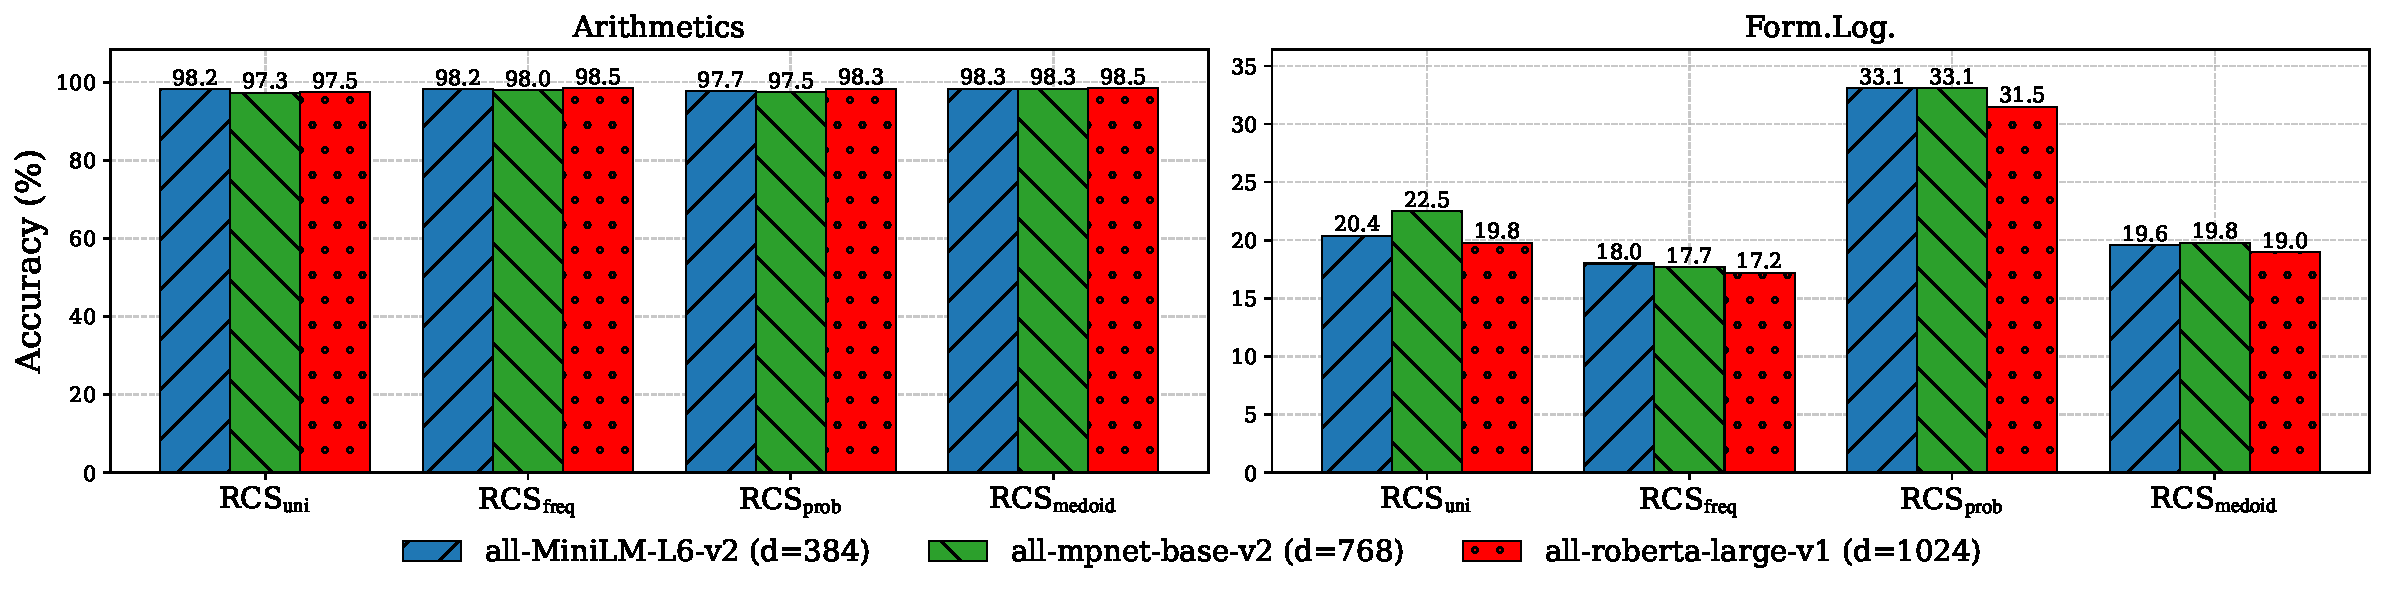
\includegraphics[width=\linewidth]{plots/abl_llama3.2-3b_embedding_v3.pdf}
    \caption{
    Effect of encoders on Llama3.2-3B. Results for Qwen2.5-3B are in Appendix Figure~\ref{fig:embed_qwen2.5-3b}.
    }
    \label{fig:embed_llama3.2-3b}
\end{figure*}

%------------
\begin{figure*}[!t]
    \centering
    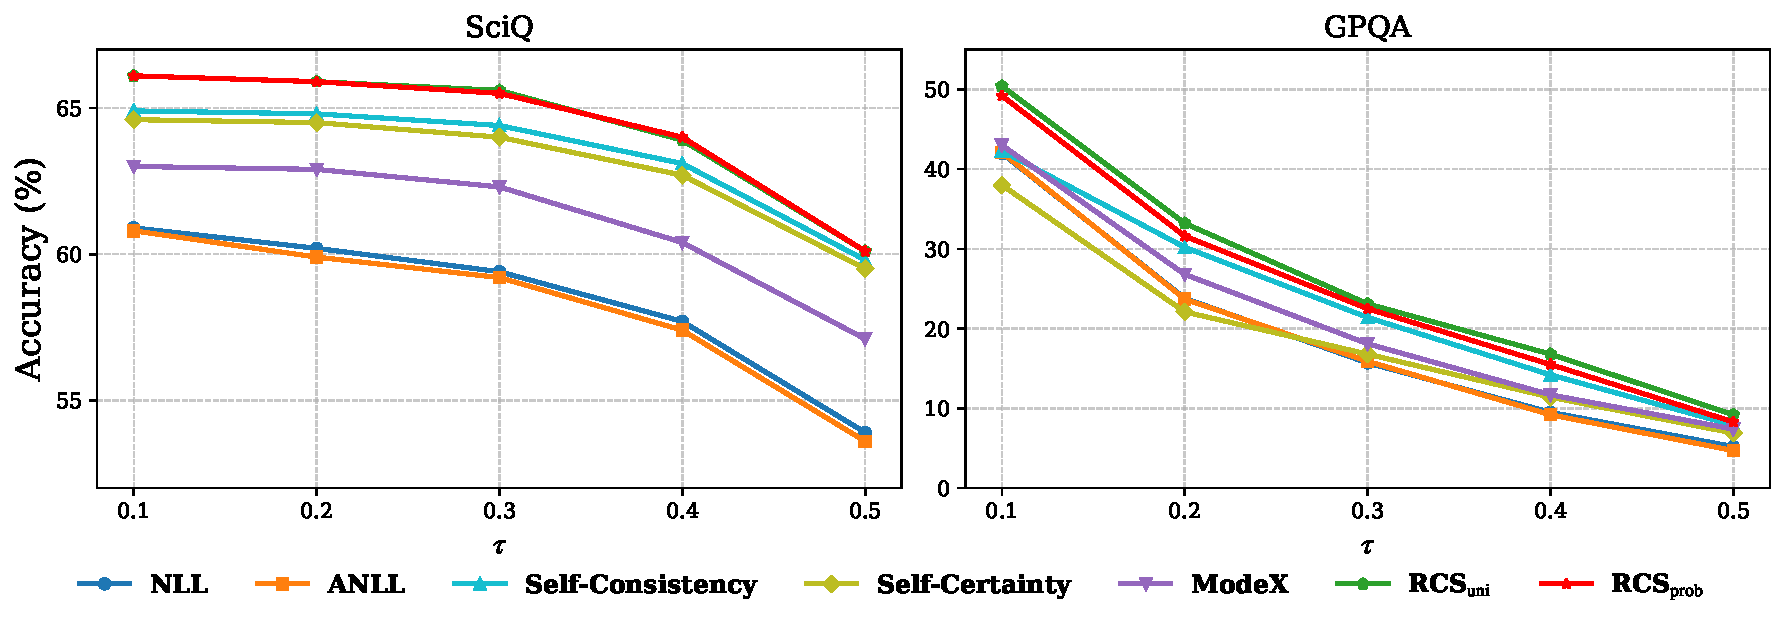
\includegraphics[width=\linewidth]{plots/abl_qwen2.5-3b_threshold_v5.pdf}
    \caption{
    Effect of varying $\tau$ using Qwen2.5-3B. Results for Llama3.2-3B are in Appendix Figure~\ref{fig:threshold_llama3.2-3b}.
    }
    \label{fig:threshold_qwen2.5-3b}
\end{figure*}
% ----------



We further evaluate RCS as a drop-in replacement for majority voting in multi-agent debate~\citep{du2023improving, choi2025debate} under a fully black-box setting with $N{=}10,20$ agents and $R{=}2$ rounds. We report RCS$_\text{base}$ and RCS$_\text{freq}$ (Table~\ref{tab:mad_qwen2.5-3b}), which are computationally efficient and do not require access to model internals.
Increasing the number of agents to $N{=}20$ consistently degrades performance across debate rounds, particularly on Llama3.2-3B, suggesting that naive scaling introduces additional variability that destabilizes reasoning~\citep{nguyen2026hear}. In contrast, RCS improves performance by 1--2\% on average, with larger gains at $N{=}20$, highlighting its robustness when aggregation becomes more challenging.

% Notably, increasing the number of agents to $N{=}20$ leads to a consistent performance drop across main debate rounds ($R{=}1,2$), particularly on Llama3.2-3B. This suggests that naively scaling up the number of agents in multi-agent debate may not always be beneficial, as it can introduce additional variability that degrades reasoning quality and destabilizes subsequent debate updates~\citep{nguyen2026hear}. 
% In contrast, RCS consistently improves performance by 1--2\% on average, with more pronounced gains at $N{=}20$, indicating its robustness in settings where answer distributions are less structured and effective aggregation becomes critical.

% \begin{table}[t]
% \centering
% \caption{Performance on Arithmetics and Form.Log. with Multi-agent Debate on Qwen2.5-3B. Best values are bolded. $R{=}0,1,2$ indicate debate rounds. Similar results for Llama3.2-3B are provided in Appendix Table~\ref{tab:mad_llama3.2-3b}.}
% \label{tab:mad_qwen2.5-3b}

% \begin{tabular}{l l|ccc}
% \toprule
% \textbf{Dataset} & \textbf{Method} & \textbf{R=0} & \textbf{R=1} & \textbf{R=2} \\
% \midrule

% \multirow{3}{*}{Arithmetics}
% & SC
% & 98.3$\pm$0.6 & 76.7$\pm$0.8 & \textbf{38.8$\pm$3.5} \\

% & RCS$_\text{base}$
% & \textbf{98.5$\pm$0.5} & \textbf{77.0$\pm$0.5} & \textbf{38.8$\pm$4.0} \\

% & RCS$_\text{freq}$
% & 98.3$\pm$0.8 & 76.7$\pm$0.6 & \textbf{38.8$\pm$3.5} \\

% \midrule

% \multirow{3}{*}{Form.Log.}
% & SC
% & 43.4$\pm$4.8 & 33.9$\pm$2.3 & 26.5$\pm$1.2 \\

% & RCS$_\text{base}$
% & \textbf{44.7$\pm$2.8} & \textbf{35.7$\pm$2.1} & 26.7$\pm$1.7 \\

% & RCS$_\text{freq}$
% & 44.4$\pm$3.2 & 35.4$\pm$2.4 & \textbf{27.0$\pm$1.6} \\

% \bottomrule
% \end{tabular}
% \end{table}

% \begin{table}[t]
% \centering
% \caption{Performance under (a) Multi-agent Debate (MAD) on Qwen2.5-3B and (b) Clean-answer setting. Best values are bolded. For MAD, $R{=}0,1,2$ indicate debate rounds and similar results for Llama3.2-3B are provided in Appendix Table~\ref{tab:mad_llama3.2-3b}. }
% \label{tab:mad_clean}

% \begin{minipage}[t]{0.45\linewidth}
% \centering
% \caption*{(a)}
% \resizebox{\linewidth}{!}{
% \begin{tabular}{l l|ccc}
% \toprule
% \textbf{Dataset} & \textbf{Method} & \textbf{R=0} & \textbf{R=1} & \textbf{R=2} \\
% \midrule

% \multirow{3}{*}{Arithmetics}
% & SC
% & 98.3$\pm$0.6 & 76.7$\pm$0.8 & \textbf{38.8$\pm$3.5} \\

% & RCS$_\text{base}$
% & \textbf{98.5$\pm$0.5} & \textbf{77.0$\pm$0.5} & \textbf{38.8$\pm$4.0} \\

% & RCS$_\text{freq}$
% & 98.3$\pm$0.8 & 76.7$\pm$0.6 & \textbf{38.8$\pm$3.5} \\

% \midrule

% \multirow{3}{*}{Form.Log.}
% & SC
% & 43.4$\pm$4.8 & 33.9$\pm$2.3 & 26.5$\pm$1.2 \\

% & RCS$_\text{base}$
% & \textbf{44.7$\pm$2.8} & \textbf{35.7$\pm$2.1} & 26.7$\pm$1.7 \\

% & RCS$_\text{freq}$
% & 44.4$\pm$3.2 & 35.4$\pm$2.4 & \textbf{27.0$\pm$1.6} \\

% \bottomrule
% \end{tabular}
% }
% \end{minipage}
% \hfill
% \begin{minipage}[t]{0.53\linewidth}
% \centering
% \caption*{(b)}
% \resizebox{\linewidth}{!}{
%   \begin{tabular}{l|cc|cc}
%     \toprule
%     \multirow{2}{*}{\textbf{Method}} 
%     & \multicolumn{2}{c|}{\textbf{Qwen2.5-3B}} 
%     & \multicolumn{2}{c}{\textbf{Llama3.2-3B}} \\
%     \cmidrule(lr){2-3} \cmidrule(lr){4-5}
%     & \textbf{Arithmetics} & \textbf{Form.Log.} 
%     & \textbf{Arithmetics} & \textbf{Form.Log.} \\
%     \midrule
%     NLL  & 54.2$\pm$4.3 & 29.6$\pm$5.6 & 87.0$\pm$1.0 & 38.6$\pm$4.4 \\
%     ANLL & 54.0$\pm$4.0 & 29.9$\pm$6.2 & 89.5$\pm$2.3 & 38.9$\pm$5.6 \\
%     SC   & 96.7$\pm$1.2 & 46.6$\pm$1.7 & 98.0$\pm$1.3 & 36.2$\pm$3.2 \\
%     CE   & 96.5$\pm$0.9 & 48.4$\pm$1.1 & 97.8$\pm$1.3 & 37.8$\pm$2.9 \\
%     \rowcolor{green!15} RCS$_{\text{medoid}}$ & \textbf{97.2$\pm$0.6} & 48.9$\pm$1.2 & 98.3$\pm$0.8 & 36.5$\pm$2.9 \\
%     \rowcolor{green!15} RCS$_{\text{uni}}$  & 95.5$\pm$1.3 & 49.2$\pm$0.8 & 98.2$\pm$1.0 & 37.0$\pm$3.3 \\
%     \rowcolor{green!15} RCS$_{\text{freq}}$ & 96.8$\pm$0.6 & \textbf{49.7$\pm$0.9} & \textbf{98.3$\pm$0.8} & 37.0$\pm$2.0 \\
%     \rowcolor{green!15} RCS$_{\text{prob}}$ & 94.3$\pm$1.9 & 48.4$\pm$0.8 & 97.7$\pm$1.0 & \textbf{40.2$\pm$4.8} \\
%     \bottomrule
%   \end{tabular}}
% \end{minipage}
% \end{table}

% \paragraph{Performance Under Clean-Answer Setting.}
% We observe that empty or degenerate responses often occur in long-form reasoning tasks. For fair comparison, we report results under a clean-answer setting, where blank or null responses are excluded from selection (Table~\ref{tab:clean-blackbox-complexity}a).
% % Removing blank answers slightly reduces performance, particularly on mathematical datasets. 
% % This suggests that blank responses are not purely noise, but may carry informative signals about model uncertainty.
% RCS-based methods remain the best-performing approaches across all settings, although the performance gap becomes smaller compared to the default setting. 
% This indicates that competing methods are more sensitive to noisy contexts, where the presence of invalid responses degrades their effectiveness more significantly.
% Notably, the advantage of RCS is more pronounced on the Form.Log., with an average improvement of around 1--2\% over the second-best method. 
% This may be attributed to the richer semantic structure of symbolic outputs (e.g. (A)), where embedding-based aggregation can better exploit high-dimensional information compared to purely numerical answers.

% \begin{table}[t]
%   \centering
%   \caption{Performance on Arithmetics and Form.Log. under clean-answer setting. Best values are bolded.}
%   \label{tab:clean}
%   % \resizebox{\columnwidth}{!}{
%   \begin{tabular}{l|cc|cc}
%     \toprule
%     \multirow{2}{*}{\textbf{Method}} 
%     & \multicolumn{2}{c|}{\textbf{Qwen2.5-3B}} 
%     & \multicolumn{2}{c}{\textbf{Llama3.2-3B}} \\
%     \cmidrule(lr){2-3} \cmidrule(lr){4-5}
%     & \textbf{Arithmetics} & \textbf{Form.Log.} 
%     & \textbf{Arithmetics} & \textbf{Form.Log.} \\
%     \midrule
%     NLL  & 54.2$\pm$4.3 & 29.6$\pm$5.6 & 87.0$\pm$1.0 & 38.6$\pm$4.4 \\
%     ANLL & 54.0$\pm$4.0 & 29.9$\pm$6.2 & 89.5$\pm$2.3 & 38.9$\pm$5.6 \\
%     SC   & 96.7$\pm$1.2 & 46.6$\pm$1.7 & 98.0$\pm$1.3 & 36.2$\pm$3.2 \\
%     CE   & 96.5$\pm$0.9 & 48.4$\pm$1.1 & 97.8$\pm$1.3 & 37.8$\pm$2.9 \\
%     \rowcolor{green!15} RCS$_{\text{medoid}}$ & \textbf{97.2$\pm$0.6} & 48.9$\pm$1.2 & 98.3$\pm$0.8 & 36.5$\pm$2.9 \\
%     \rowcolor{green!15} RCS$_{\text{uni}}$  & 95.5$\pm$1.3 & 49.2$\pm$0.8 & 98.2$\pm$1.0 & 37.0$\pm$3.3 \\
%     \rowcolor{green!15} RCS$_{\text{freq}}$ & 96.8$\pm$0.6 & \textbf{49.7$\pm$0.9} & \textbf{98.3$\pm$0.8} & 37.0$\pm$2.0 \\
%     \rowcolor{green!15} RCS$_{\text{prob}}$ & 94.3$\pm$1.9 & 48.4$\pm$0.8 & 97.7$\pm$1.0 & \textbf{40.2$\pm$4.8} \\
%     \bottomrule
%   \end{tabular}
%   % }
% \end{table}


\paragraph{RCS Improves Under Fully Black-box Setting.}
We further evaluate a fully black-box setting using Cohere (\textit{command-a-03-2025}) on GPQA, MMLU-Pro, and BigBenchHard (Table~\ref{tab:clean-blackbox-complexity}a). RCS outperforms traditional Self-Consistency, with RCS$\text{base}$ achieving the best performance, yielding +1\% average improvement. This highlights the advantage of RCS in capturing consistency beyond simple frequency-based selection.

% \begin{table}[t]
%   \centering
%   \caption{Performance across methods under fully blackbox setting. Best values are bolded.}
%   \label{tab:blackbox}
%   % \resizebox{\columnwidth}{!}{
%   \begin{tabular}{l|cc}
%     \toprule
%     {\textbf{Method}} 
%     & {\textbf{AIME25}} 
%     & {\textbf{MMLU-Pro}} \\
%     \midrule
%     SC  & \textbf{6.7} & 47.6 \\
%     \rowcolor{green!15} RCS$_\text{medoid}$& \textbf{6.7} & \textbf{48.6} \\
%     \rowcolor{green!15} RCS$_\text{base}$ & \textbf{6.7} & \textbf{48.6} \\
%     \rowcolor{green!15} RCS$_\text{freq}$   & \textbf{6.7} & 47.6 \\
%     \bottomrule
%   \end{tabular}
%   % }
% \end{table}

% \begin{table}[t]
% \centering
% \caption{Complexity comparison (a) and performance under fully black-box setting (b).}
% \label{tab:complexity_blackbox}

% \begin{minipage}[t]{0.48\linewidth}
% \centering
% \caption*{(a)}
% \begin{tabular}{l|cc}
% \toprule
% \textbf{Method} & \textbf{AIME25} & \textbf{MMLU-Pro} \\
% \midrule
% SC & 6.7 & 47.6 \\
% RCS$_\text{medoid}$ & 6.7 & \textbf{48.6} \\
% RCS$_\text{base}$ & 6.7 & \textbf{48.6} \\
% RCS$_\text{freq}$ & 6.7 & 47.6 \\
% \bottomrule
% \end{tabular}
% \end{minipage}
% \hfill
% \begin{minipage}[t]{0.48\linewidth}
% \centering
% \caption*{(b)}
% \begin{tabular}{l c}
% \toprule
% \textbf{Method} & \textbf{Complexity} \\
% \midrule
% NLL, ANLL, SC & $\mathcal{O}(N)$ \\
% % Self-Consistency (SC) & $\mathcal{O}(N)$ \\
% Self-Certainty (CE) & $\mathcal{O}(N L V)$ \\
% RCS$_\text{medoid}$ & $\mathcal{O}(N^2 d)$ \\
% RCS$_\text{uni/freq/prob}$ & $\mathcal{O}(N d)$ \\
% \bottomrule
% \end{tabular}
% \end{minipage}
% \end{table}

\paragraph{Complexity Analysis.}\label{sec:complexity}

We report computational complexity in Table~\ref{tab:clean-blackbox-complexity}b, where $d$, $L$, and $|V|$ denote embedding dimension, sequence length, and vocabulary size.
NLL and ANLL scale as $\mathcal{O}(NL)$ due to token-level scoring, while SC is $\mathcal{O}(N)$ since it only performs frequency counting over final answers. More expressive methods such as CE and ModeX capture richer semantic or structural dependencies but incur higher costs due to full token-level distributions or pairwise interactions.
In contrast, RCS variants (e.g., RCS$_\text{uni}$) avoid pairwise comparisons by estimating a semantic center and dispersion in $\mathcal{O}(Nd)$, achieving a favorable trade-off between efficiency and semantic expressiveness.

\paragraph{Qualitative Example.}\label{sec:qualitative}
We present two qualitative examples from Arithmetics and Form.Log. (Figure~\ref{fig:qualitative}), using $N{=}5$ samples for Self-Consistency and RCS$_\text{uni}$ for simplicity. 
Self-Consistency fails when majority responses are misleading, whereas RCS$_\text{uni}$ correctly recovers the answer by leveraging informative minority samples. This highlights the robustness of RCS in aggregating diverse outputs under noisy sampling.


% \begin{table}[t]
% \centering
% \caption{Computational complexity comparison. $N$ is the number of samples, $d$ is the embedding dimension, $L$ is the sequence length, and $V$ is the vocabulary size.}
% \label{tab:complexity}
% \begin{tabular}{l c}
% \toprule
% \textbf{Method} & \textbf{Complexity} \\
% \midrule
% NLL, ANLL & $\mathcal{O}(N)$ \\%& Per-sequence likelihood scoring \\
% Self-Consistency (SC) & $\mathcal{O}(N)$ \\%& Frequency counting \\
% Self-Certainty (CE) & $\mathcal{O}(N L V)$ \\%& Token-level distributions + aggregation \\
% RCS$_\text{medoid}$ & $\mathcal{O}(N^2 d)$ \\%& Pairwise distances \\
% RCS$_\text{uni}$, RCS$_\text{freq}$, RCS$_\text{prob}$ \\%& $\mathcal{O}(Nd)$ & Center + distances in embedding space \\
% \bottomrule
% \end{tabular}
% \end{table}


% ============
% \begin{figure*}[t]
%     \centering

%     \begin{minipage}[t]{0.51\linewidth}
%         \centering
%         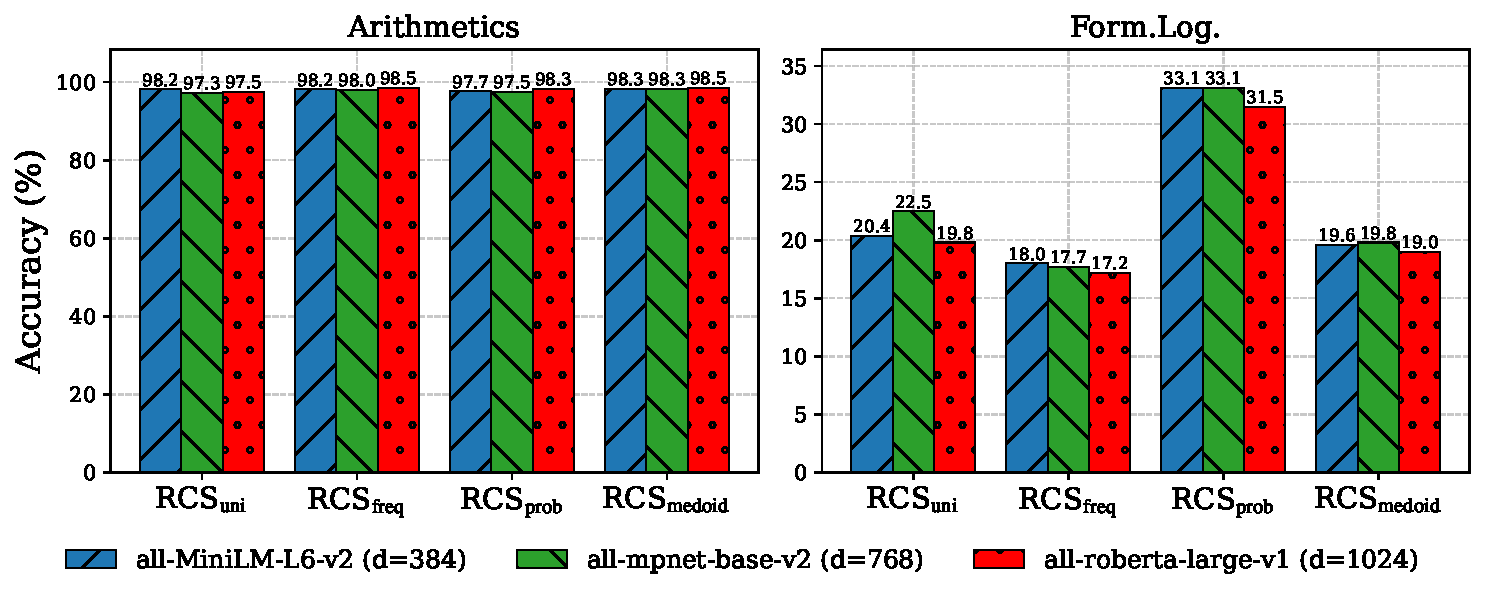
\includegraphics[width=\linewidth]{plots/abl_llama3.2-3b_embedding_v4.pdf}
%         \caption*{(a)}
%     \end{minipage}
%     \hfill
%     \begin{minipage}[t]{0.48\linewidth}
%         \centering
%         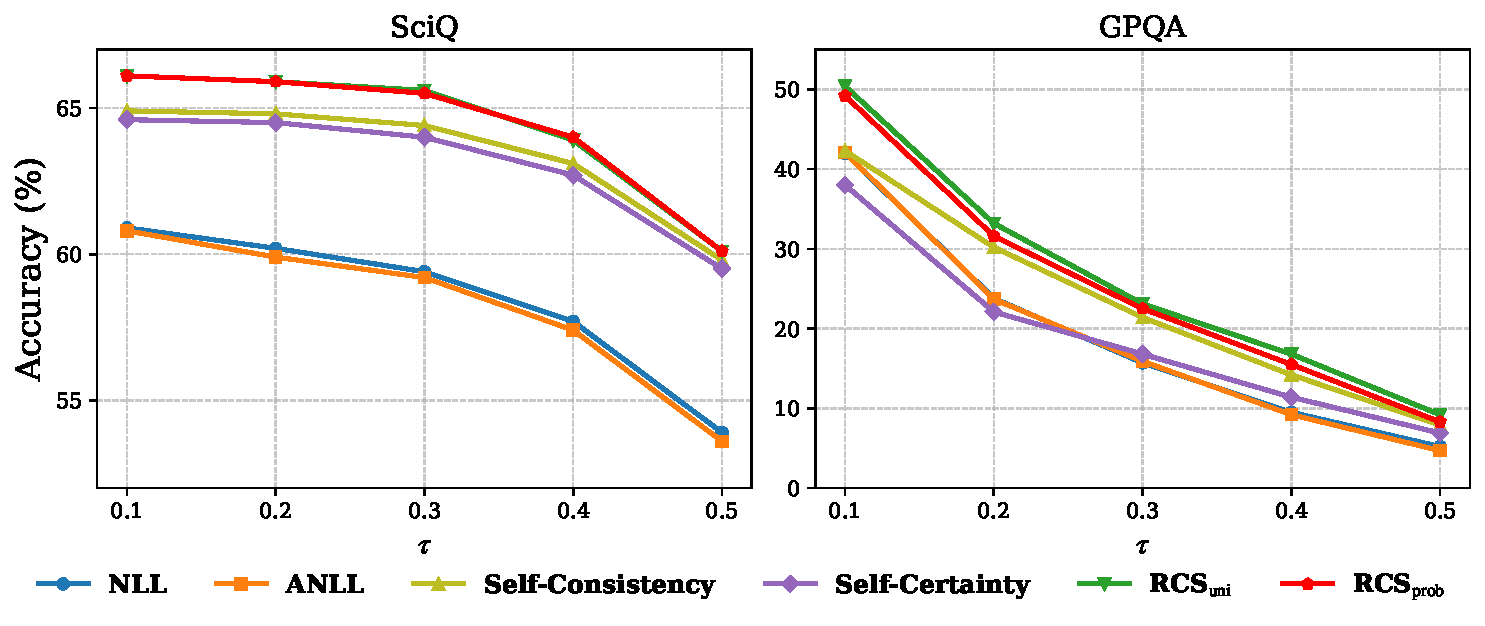
\includegraphics[width=\linewidth]{plots/abl_qwen2.5-3b_threshold_v4.pdf}
%         \caption*{(b)}
%     \end{minipage}

%     \caption{
%     (a) Effect of the sentence embedding model on Arithmetics and Form.Log. using Llama3.2-3B. 
%     (b) Performance on SciQ and GPQA when varying correctness threshold ($\tau$) using Qwen2.5-3B. 
%     Additional results are provided in Appendix Figures~\ref{fig:embed_qwen2.5-3b} and~\ref{fig:threshold_llama3.2-3b}.
%     }
%     \label{fig:embed_threshold}
% \end{figure*}
\paragraph{Analysis Of Design Choices.}
We analyze the impact of several design choices in RCS. 
% and provide qualitative examples to further illustrate its behavior. 
% \textbf{(1) Qualitative Example.}\label{sec:qualitative} We present two qualitative examples from Arithmetics and Form.Log. (Figure~\ref{fig:qualitative}), using $N{=}5$ samples for Self-Consistency and RCS$_\text{uni}$ for simplicity. 
% Self-Consistency fails when majority responses are misleading, whereas RCS$_\text{uni}$ correctly recovers the answer by leveraging informative minority samples. This highlights the robustness of RCS in aggregating diverse outputs under noisy sampling.
\textbf{(1) Effect Of Embedding Models:} In Figure~\ref{fig:embed_llama3.2-3b}, we compare three sentence transformers of increasing capacity. 
% : \texttt{all-MiniLM-L6-v2}, \texttt{all-mpnet-base-v2}, and \texttt{all-roberta-large-v1}. 
Results show minimal variation across models. This stability is especially evident on Arithmetics, where answers are numeric. On Form.Log., we observe a slight drop with \texttt{all-roberta-large-v1}, particularly for the probability-based variant, suggesting that higher embedding capacity does not necessarily improve semantic alignment in this setting. \textbf{(2) Effect Of Correctness Threshold:} Figure~\ref{fig:threshold_qwen2.5-3b} reports performance on SciQ and GPQA under varying correctness thresholds. We focus on \textsc{RCS}$_{\text{uni}}$ and \textsc{RCS}$_{\text{prob}}$, which consistently achieve the best results as the ROUGE-F1 threshold increases from 0.1 to 0.5, particularly within the common range of 0.2--0.4. 
% This demonstrates RCS's robustness to threshold selection. 
\textbf{(3) Effect of Full-Trajectory Embeddings:}\label{sec:embedding-collapse} A natural extension of RCS is to use full generation trajectories instead of final-answer embeddings. However, this leads to an \textit{embedding collapse} effect, where candidates become less distinguishable due to shared prefixes and redundant reasoning.
We compare this variant with final-answer embeddings (Appendix Figures~\ref{fig:full_qwen2.5-3b} and~\ref{fig:full_llama3.2-3b}) and observe consistent performance drops. This suggests that intermediate tokens introduce noise and weaken discriminative signals, while final answers provide a more compact and task-relevant representation. % These results support our design choice.
This collapse issue also affects methods that operate on full trajectories: ModeX applies spectral clustering over complete reasoning traces, while SCW~\citep{jain2023sc} embeds full reasoning paths and groups pairwise cosine-similarity scores by unique trajectory. Although SCW's similarity-based aggregation provides an implicit outlier-down-weighting effect, shared prefixes still cause representations to collapse, and the discrete grouping-by-trajectory step can miss minority correct answers. RCS avoids both issues by restricting embeddings to the extracted final answer and ranking all candidates continuously via the weighted Fréchet mean.

% \paragraph{Effect Of Embedding Models.}

% In Figure~\ref{fig:embed_llama3.2-3b}, we compare three sentence transformers of increasing capacity: \texttt{all-MiniLM-L6-v2}, \texttt{all-mpnet-base-v2}, and \texttt{all-roberta-large-v1}. Results show minimal variation across models. This stability is especially evident on Arithmetics, where answers are numeric. On Form.Log., we observe a slight drop with \texttt{all-roberta-large-v1}, particularly for the probability-based variant, suggesting that higher embedding capacity does not necessarily improve semantic alignment in this setting.

% \paragraph{Effect Of Correctness Threshold.}

% Figure~\ref{fig:threshold_qwen2.5-3b} reports performance on SciQ and GPQA under varying correctness thresholds. We focus on \textsc{RCS}$_{\text{uni}}$ and \textsc{RCS}$_{\text{prob}}$, which consistently achieve the best results as the ROUGE-F1 threshold increases from 0.1 to 0.5, particularly within the common range of 0.2--0.4. This demonstrates RCS's robustness to threshold selection.

% % Figure~\ref{fig:threshold_qwen2.5-3b} reports performance on SciQ and GPQA under varying correctness thresholds. We focus on \textsc{RCS}$_{\text{uni}}$ and \textsc{RCS}$_{\text{prob}}$, the two best-performing variants among our methods. As the ROUGE-F1 threshold increases from 0.1 to 0.5, both variants consistently achieve the strongest results across datasets, particularly within the commonly used range of 0.1–0.4. This demonstrates the robustness of our approach to threshold selection. 
% % Full results are provided in Appendix Table~\ref{tab:threshold_full}.


% \paragraph{Effect of Full-Trajectory Embeddings.}\label{sec:embedding-collapse}

% A natural extension of RCS is to use full generation trajectories instead of final-answer embeddings. However, this leads to an \textit{embedding collapse} effect, where candidates become less distinguishable due to shared prefixes and redundant reasoning.
% We compare this variant with final-answer embeddings (Appendix Figures~\ref{fig:full_qwen2.5-3b} and~\ref{fig:full_llama3.2-3b}) and observe consistent performance drops. This suggests that intermediate tokens introduce noise and weaken discriminative signals, while final answers provide a more compact and task-relevant representation. These results support our design choice.